\documentclass[13pt, a4paper, twoside]{article}
\usepackage[utf8]{inputenc}
\usepackage{geometry}
\usepackage[czech]{babel}
\usepackage{chemformula}
\usepackage{chemfig}
\usepackage{float}
\usepackage{caption}
\usepackage{enumitem}
\usepackage{fancyhdr}
\usepackage{setspace}
\usepackage{multicol}
\geometry{legalpaper, margin=1in}
\pagestyle{fancy}
\lhead{\Large Šárka Doležalová, skupina 6}
\rhead{\large 10.12.2020}
\begin{document}
    \begin{center}
        \Huge
        Úloha 5: Spektrofotometrická kvantitativní analýza
    \end{center}
    \onehalfspacing \large
    \section*{Zadané úlohy}
    \begin{enumerate}
        \item Sestrojte kalibrační křivku pro spektrofotometrické stanovení koncentrace měďnatých
        iontů.
        \item Stanovením obsahu mědi v neznámém pevném materiálu identifikujte, o jakou sloučeninu
        se jedná.
    \end{enumerate}
    \section*{Teoretický úvod}
    Zařízení, které je využíváno k vypracování této úlohy se nazývá spektrometr.
    Tento přístroj je založen na získvávání monochormatického záření, které vypovídá
    po průchodu zkoumannou látkou různou intenzitu. V našem případě je použit pro
    měření absorbance dvoupaprskový spektrofotometrem, ve kterém prochází záření blankem
    (provnávacím roztokem) a měřeným vzorkem najednou. K dorpavení fotonů do násobiče
    je postaránou soustavou zrcadel. Kyvety, kteréžto jsou použity pro roztoky nesmějí
    absorbovat záření v stanoveném vlnovém rozsahu.


    Lambertův-Beerův zákon je vztah mezi absobancí, koncentrací vzorku a absorbujícího prostředí
    (šírka kyvety). $A_{\lambda}=\epsilon_{\lambda} \cdot c \cdot l$, kde $\epsilon_{\lambda}$
    je absorbční koeficient, který je konstantní pro danou látku při vlnové délce záření $\lambda$.
    Platnost tohoto zákona se ověřuje experimentálně, tak že jsou vyneseny hodnoty absorbance naproti
    naproti koncentrací roztoků. Vynesené bodu se následně lineárně interpolují a vznikne kalibrační křivka.

    

    \section*{Postup}
    \subsection*{Příprava standardních roztoků modré skalice}
    Bylo označeno pět 10ml odměrných baněk. Do připravených baněk bylo odpipetováno 
    spočítané množství $CuSO_4$ (c=0,150) tak, aby byla kádince koncentrace 0,005, 0,010,
    0,015, 0,020 a 0,025 M a dolity destilovanou vodou na objem 10 ml. Roztoky v odměrných 
    baňkách byly pořádně promíchány. Připravené roztoky byly přelity do lékovek označených 
    CuA–CuE. Odsud bylo pomocí automatické pipety přeneseno množství 5,00 ml do nových
    lékovek popsaných CuST1–CuST5 a poté k nim přidáno 1,00 ml 5\% vodného roztoku
    amoniaku. Lékovky byly pečlivě uzavřeny a promíchány. Bylo pozorováno, že roztok se zbarvil do výrazně modré. 

    \begin{figure}[H]
        \centering
        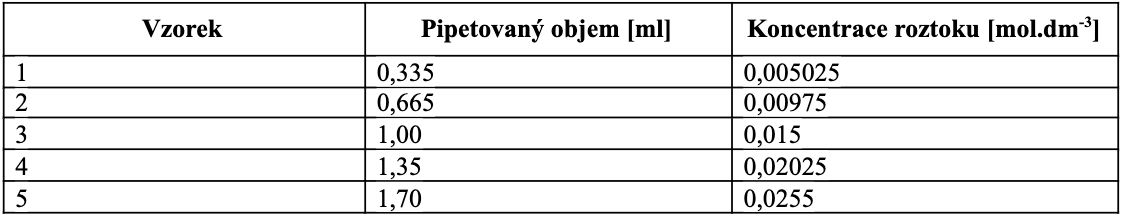
\includegraphics[width=6.5in]{uloha_5_tab_1.png}
        \caption*{Tab. 1: pipetovaný objem a koncentrace vzorků}
    \end{figure}

    \subsection*{Příprava roztoku neznámého vzorku}
    Bylo odváženo 74,7 mg neznámého roztoku číslo 56. Vzorek byl rozpuštěn v destilované vodě v 25 ml odměrné baňce. Z roztoku bylo pipetou odebráno 5,00 ml a poté smícháno s 1,00 ml 5\% roztoku amoniaku.

    \subsection*{Příprava referenčního roztoku}
    Do lékovky bylo odpipetováno 5,00 ml vody a do něj bylo přidáno 1,00 ml 5\% roztoku amoniaku.

    \subsection*{Zjištění optimální vlnové délky pro měření}
    Do dvou vypláchnutých kyvet byl vnesen referenční roztok tak, aby hladina byla cca 6 mm pod jejich horním okrajem a kyvety byly vsunuty do přístroje. Nejdříve bylo provedeno „reference“ měření pomocí referenčního roztoku, poté „measure“ měření se stejným roztokem. Takto byla stanovena nulová hodnota absorbance. Dále byla kyveta vypláchnuta a naplněna nejkoncentrovanějším roztokem modré skalice, na základě měření bylo zjištěno absorpční maximum při vlnové délce 603 nm, viz graf Absorpční spektrum amoniakálního roztoku modré skalice.

    \begin{figure}[H]
        \centering
        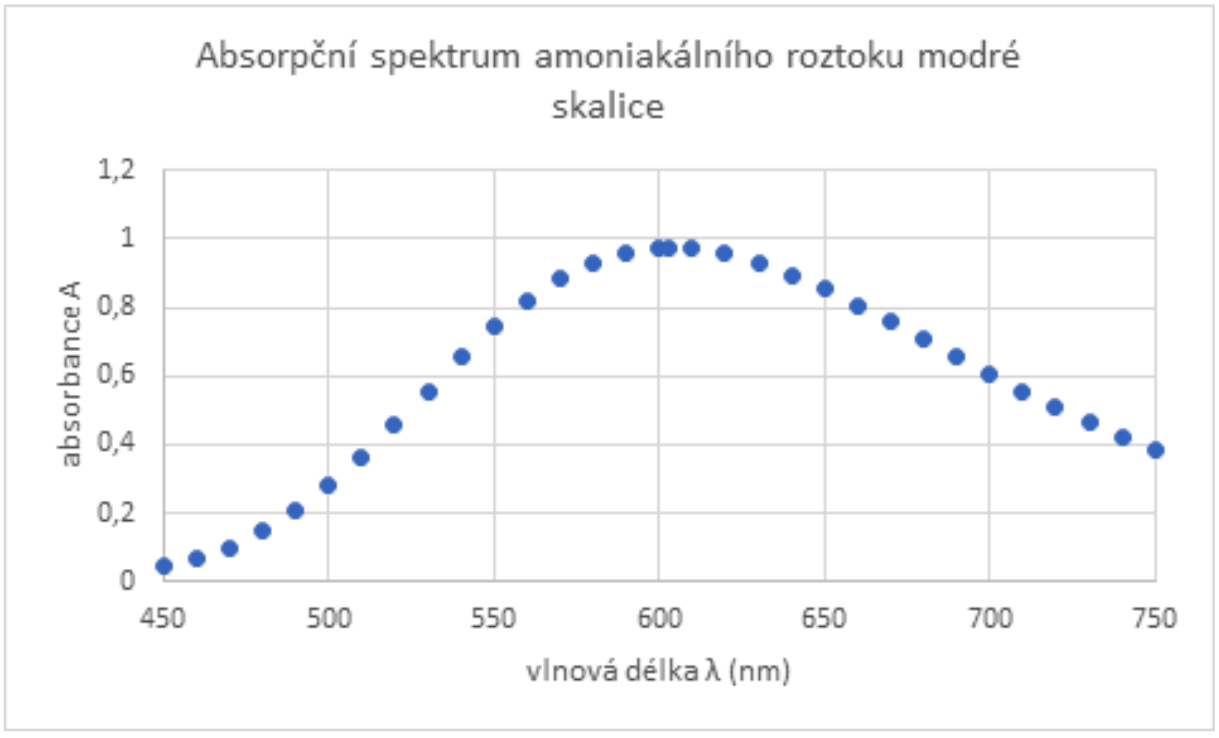
\includegraphics[width=6.5in]{uloha_5_graf_1.png}
    \end{figure}

    \subsection*{Sestrojení kalibrační křivky}
    Dále byly naměřeny hodnoty absorbance jednotlivých roztoků při vlnové délce rovnající se 603 nm. Podle naměřených hodnot vynesena kalibrační křivka s ve tvaru regresní rovnice:
    \begin{figure}[H]
        \centering
        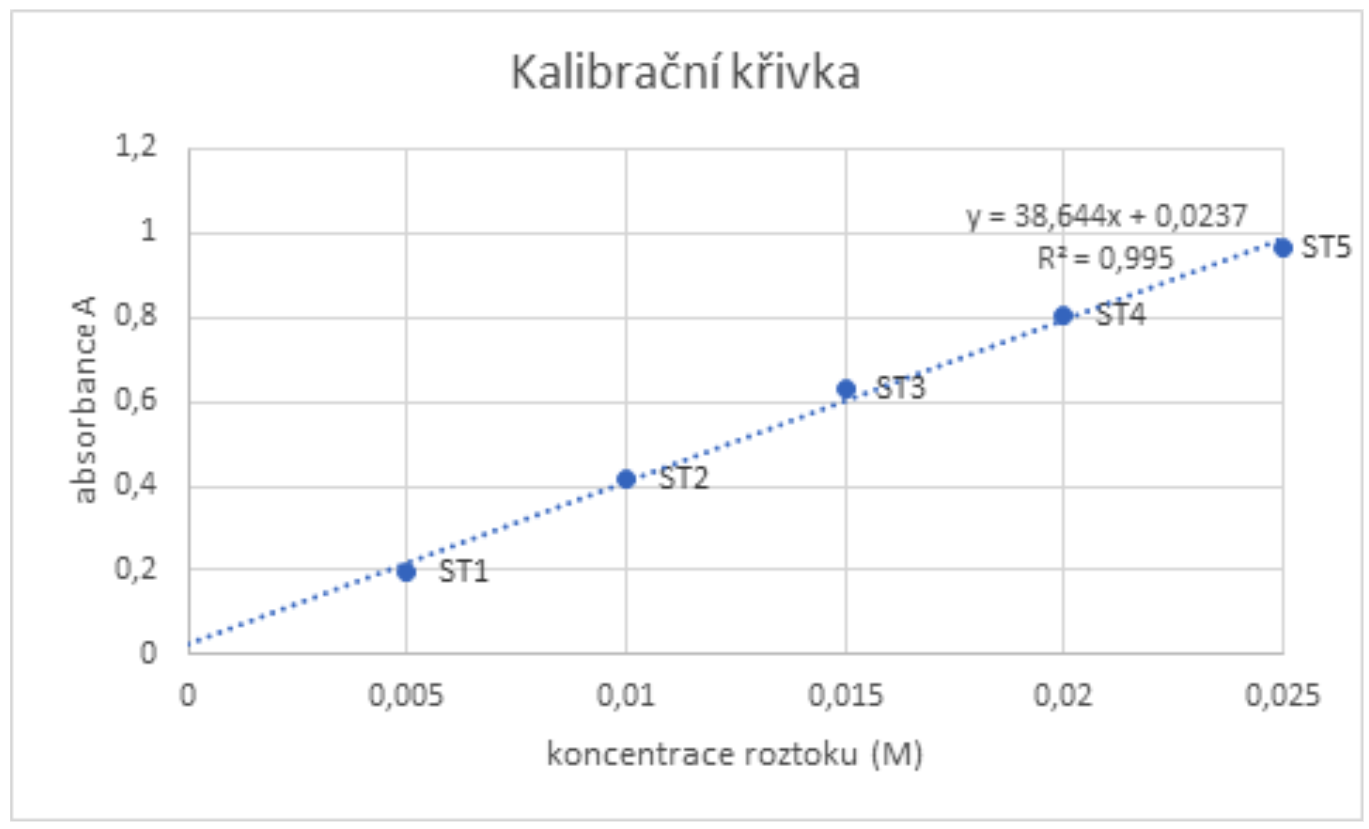
\includegraphics[width=6.5in]{uloha_5_graf_2.png}
    \end{figure}

    \section*{Naměřené hodnoty}
    \begin{figure}[H]
        \centering
        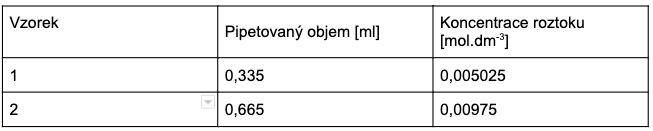
\includegraphics[width=6.5in]{uloha_5_tab_2.png}
        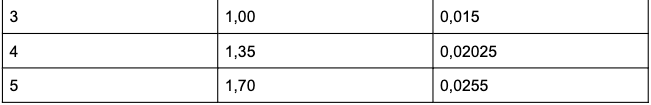
\includegraphics[width=6.5in]{uloha_5_tab_3.png}
        \caption*{Tab. 2: pipetovaný objem a koncentrace roztoků}
    \end{figure}

    \begin{figure}[H]
        \centering
        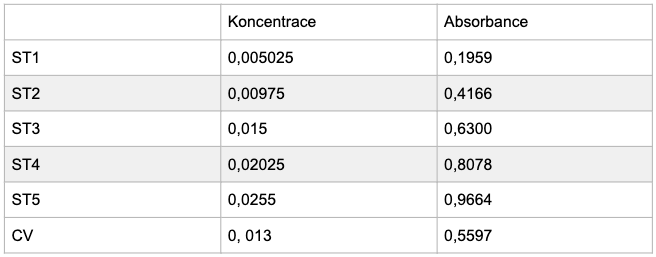
\includegraphics[width=6.5in]{uloha_5_tab_4.png}
        \caption*{Tab. 3: Absorbance vzorků}
    \end{figure}

    \section*{Výpočty}
    \subsection*{Molární koncentrace vzorků}
    \begin{align*}
        A_{(CV)} &= 0,5597 \\
        y &= 38,644 \cdot 0,0237 \\
        \to y&=A \\
        \to x&=c \\
        V_{(CV)} &= 0,025 dm^3 \\
        \to c&= \frac{A-0,0237}{38,644}\\
        c&=0,0139 \: M
    \end{align*}

    \subsection*{Látkové množství}
    \begin{align*}
        n=c\cdot V\\
        n=3,48 \cdot 10^{-4} \: mol
    \end{align*}

    \subsection*{Molární hmotnost}
    \begin{align*}
        M_{(CV)}=\frac{m}{n}\\
        M_{(CV)} = 214,65 \: g \cdot mol^{-1}
    \end{align*}

    \subsection*{Hmotnostní zlomek}
    \begin{align*}
        \omega = \frac{c\cdot V \cdot M_{Cu}}{m}\\
        \omega = 0,30
    \end{align*}

    \subsection*{Extinkční koeficient}
    \begin{align*}
        A_{(603\:nm)} &= 0,9664 \\
        c &= 0,0255\: M \\
        l = 1\: cm\\
        \to \epsilon_{(603\: nm)} &= \frac{A_{(603\:nm)}}{c \cdot l}\\
        \epsilon_{(603\: nm)} &= 36,90 \: dm^3 \cdot cm^{-1} \cdot mol^{-1}
    \end{align*}

    \section*{Závěr}
    Neznámý vzorek byl s pomocí kalibrační křivky identifikován jako $CuBr_2$. Dále byl spočítán extinkční koeficient v absorpčním maximu $\epsilon_{(603\: nm)} = 36,90 \: dm^3 \cdot cm^{-1} \cdot mol^{-1}$.


\end{document}